\documentclass[titlepage=firstcover, captions=tableheading]{scrartcl}
\usepackage{microtype}
\usepackage{amsmath}
\usepackage{polyglossia}
\usepackage{graphicx}
\usepackage{booktabs}
\usepackage{siunitx}
\usepackage{hyperref}
\usepackage{caption}
\usepackage{float}
\setdefaultlanguage{german}
\title{US3 Dopplersonographie}
\author{
Connor Magnus Böckmann \\ email: \href{mailto:connormagnus.boeckmann@tu-dortmund.de}{connormagnus.boeckmann@tu-dortmund.de}
\and Tim Theissel \\ email: \href{mailto:tim.theissel@tu-dortmund.de}{tim.theissel@tu-dortmund.de}}
\begin{document}
\maketitle
\newpage
\tableofcontents
\newpage
\section{Zielsetzung}
In diesem Versuch wird die Stroemungsgeschwindigkeit und das Stroemungsprofil durch ein System mit Hilfe von Dopplersonographie gemessen und ausgewertet werden. 
\section{Theoretische Grundlagen}
\subsection{Der Doppler-Effekt}
Der Doppler-Effekt beschreibt die Frequenzaenderung, welche auftritt, sollten sich die Quelle der Welle und der Beobachter relativ zueinander bewegen. Die Frequenz $\nu_0$ erhoeht sich zu $\nu_kl$, wenn sich die Quelle auf den Beobachter hinzu bewegt. Im Umkehrschluss verringert sich $\nu_0$ zu $\nu_{gr}$, wenn sich die Quelle und der Beobachter voneinander entfernen.\\
Wenn sich die Quelle mit der Geschwindigkeit $v$ bewegt und der Beobachter still steht, ergibt sich:
\begin{equation}
    \nu_{kl/gr}=\frac{\nu_0}{1\mp\frac{v}{c}}
\end{equation}
Sollte sich der Beobachter bewegen und die Quelle stillstehen, ergibt sich dafuer nun:
\begin{equation}
    \nu_{kl/gr}=\nu_0(1\pm\frac{v}{c})
\end{equation}
\subsection{Anwendung in der Ultraschalltechnik}
Der Doppler-Effekt kann genutzt werden, um Stroemungsgeschwindigkeiten durch ein System- zum Beispiel die Stroemungsgeschwindigkeit des Blutes durch Adern- zu messen. Die Frequenz der ausgesendetet Ultraschallwelle wird an einem Koerper, etwa an einem Blutkoerper, verschoben und reflektiert. In diesem Fall ergibt sich die Frequenzverschiebung $\Delta\nu$ mit der Geschwindigkeit des Koerpers $v$, der Schallgeschwindigkeit $c$ und den Winkeln $\alpha$ und $\beta$ zu:
\begin{equation}
    \Delta\nu=\nu_0\frac{v}{c}(\cos\alpha+\cos\beta)
\end{equation}
Das hier verwendete Impuls-Echo-Verfahren legt den Winkel der einlaufenden Welle $\alpha$ und der ruecklaufenden Welle $\beta$ auf $\alpha=\beta$. Es entsteht also folgende Formel zur Berechnung der Frequenzverschiebung:
\begin{equation}
    \Delta\nu=2\nu_0\frac{v}{c}\cos\alpha \label{4}
\end{equation} \newpage
\subsection{Die Erzeugung von Ultraschall}
Eine der moeglichen Methoden zur Erzeugung von Ultraschall ist der piezo-elektrische Effekt. Ein elektrisches Wechselfeld regt dabei einen piezo-elektrischen Kristall zu Schwingungen an. Voraussetzung ist dafür, dass eine polare Achse des kristalls in Richtung des E-Feldes zeigt. Sollte die Anregungsfrequenz mit der Eigenfrequenz des Kristalls uebereinstimmen, resoniert dieser Kristall und es koennen grosse Amplituden der Schwingungen erzeugt werden.
Umgekehrt ist dieser Piezokristall auch als Empfaenger nutzbar, wenn Schallwellen den Kristall in Schwingung versetzen. Die am haeufigsten verwendeten Kristalle sind dabei Quarze, welche aber einen relativ schwachen Piezoeffekt haben. Sowohl der Empfaenger, als auch der Sender der Ultraschallwelllen sind in der im Versuch verwendeten Sonde enthalten. 
\section{Aufbau}
Der Versuchsaufbau besteht im wesentlichen aus einem Ultraschallgenerator mit integrierter Ultraschallsonde und einem Strömungskreislauf. Die Sonde ist an einen Computer angeschlossen, welcher zur Analyse und Datenaufnahme verwendet wird. Die Strömungsröhren sind mit einer Fluessigkeit aus Wasser, Glycerin und kleinen Glaskugeln gefuellt. Diese dienen als Reflektionskoerper. Die Fliessgeschwindigkeit kann an der angeschlossenen Pumpe zwischen 0-7 l/min eingestellt werden. Die Viskositaet ist so eingestellt, dass sich in den Roehren ein laminarer Fluss bildet.
\section{Durchfuehrung}
Die Strömungsgeschwindigkeit und das Stroemungsprofil werden an drei verschiedenen Röhren (7mm, 10mm, 16mm Innendurchmesser) ermittelt. Zur Messung werden so genannte Doppler-Prismen benoetigt, welche je drei verschiedene Einschallwinkel haben. Jeder Rohrdurchmesser hat dabei ein eigenes passendes Prisma. Dadurch wird die Reproduzierbarkeit gewaehrleistet, da so der Abstand zur Fluessigkeit und der Einschallwinkel immer gleich sind.\\
Der so genannte Doppler-Winkel $\alpha$ berechnet sich aus dem Brechungsgesetz mit der Schallgeschwindigkeit in der Fluessigkeit $c_L$ und der Schallgeschwindigkeit im Prismenmaterial $c_P$ zu:
\begin{equation}
    \alpha=90^\circ-\arcsin(\sin\theta*\frac{c_L}{C_P})
\end{equation}
\subsection{Bestimmung der Dopplerverschiebung}
Zur Bestimmung der Dopplerverschiebung wird das Geraet auf SAMPLE VOLUME LARGE gestellt. Nun werden fuer jedes der drei Stroemungsrohre je fuenf Pumpleistungen eingestellt und mit dem passenden Prisma die drei Winkel durchgemessen. Der Computer gibt je eine Angabe fuer die Stroemungsgeschwindigkeit aus, mit der nun mit Hilfe von \ref{4} die Dopplerverschiebung errechnet werden kann.
\subsection{Bestimmung des Stroemungsprofils}
Zur Bestimmung des Stroemungsprofils wird das Geraet auf SAMPLE VOLUME SMALL gestellt, um die Messtiefe variieren zu koennen. Die genannte Messtiefe ist dabei in [$\mu s$] angegeben. In Acryl entspricht eine Messtiefe von $4\mu s=10mm$, wohingegen $4\mu s=6mm$ in der Dopplerfluessigkeit entsprechen. Mit einem Prismavorlauf von 30.7mm und einer Wandstaerke des gemessenen Rohrs von 2mm ergibt sich eine Mindestmesstiefe von $13.08\mu s$, um mit der Messung bis in die Fluessigkeit zu gelangen. Da das Rohr einen Innendurchmesser von 16mm hat, liegt der Bereich der Messtiefe zwischen $13.08\mu s$ und $23.75\mu s$, bis die gesamte Fluessigkeit durchgemessen wurde.

\section{Auswertung}

\subsection{Dopplerverschiebung}

Die bereits beschriebene Vorgehensweise zur Bestimmung der Dopplerverschiebung liefert die in den Tabellen \ref{tab:1}, \ref{tab:2}, \ref{tab:3} zu findenen Werte.

\noindent Werden diese Werte nun in \ref{4} eingesetzt ergeben sich folgende Werte für die Dopplerverschiebung:

\begin{minipage}{\linewidth}
    \begin{table}[H]
        \centering
    
    \begin{tabular}{lrll}
        \toprule
        Pumpgeschwindigkeit [L/min] & Prismawinkel 15$^{\circ}$ & 30$^{\circ}$ & 60$^{\circ}$ \\
        \midrule
        2.5   & 60.97  & 97.78   & 159.09  \\ 
        3     & 73.24  & 134.07  & 219.39  \\ 
        3.5   & 85.51  & 171.11  & 292.52   \\ 
        4     & 110.05 &  207.41 & 365.66  \\
        4.5   & 134.20 & 268.89  & 451.62  \\    
        \bottomrule
        
    \end{tabular}
    \captionof{table}{Frequenzverschiebung in einem Rohr mit Innendurchmesser 10mm}
    \label{tab:0}
    \end{table}
    \end{minipage}

    \begin{minipage}{\linewidth}
        \begin{table}[H]
            \centering
        
        \begin{tabular}{lrll}
            \toprule
            Pumpgeschwindigkeit [L/min] & Prismawinkel 15$^{\circ}$ & 30$^{\circ}$ & 60$^{\circ}$ \\
            \midrule
            2.5  & 48.70 & 60.74 & 85.96 \\ 
            3    & 48.70 & 73.33 & 110.34 \\ 
            3.5  & 48.70 & 85.19 & 134.72 \\ 
            4    & 61.00 & 97.78 & 170.64 \\
            4.5  & 73.24 & 122.22 & 207.85 \\    
            \bottomrule
            
        \end{tabular}
        \captionof{table}{Frequenzverschiebung in [Hz] in einem Rohr mit Innendurchmesser 16mm}
        \label{tab:5}
        \end{table}
        \end{minipage}

        \begin{minipage}{\linewidth}
            \begin{table}[H]
                \centering
            
            \begin{tabular}{lrll}
                \toprule
                Pumpgeschwindigkeit [L/min] & Prismawinkel 15$^{\circ}$ & 30$^{\circ}$ & 60$^{\circ}$ \\
                \midrule
                2.5   & 121.93 & 195.56 & 329.73 \\ 
                3     & 158.74 & 268.89 & 513.20  \\ 
                3.5   & 195.17 & 341.48 & 635.09 \\ 
                4     & 243.87 & 439.26 & 794.18  \\
                4.5   & 305.21 & 537.04 & 990.48  \\    
                \bottomrule
                
            \end{tabular}
            \captionof{table}{Messwerte für Strömungsgeschwindigkeiten in [cm/s] in einem Rohr mit Innendurchmesser 10mm}
            \label{tab:6}
            \end{table}
            \end{minipage}

\noindent Diese berechneten Werte werden nun graphisch dargestellt. Es folgen drei Grafiken in denen die Frequenzverschiebung von verschiedenen Rohrinnendurchmessern dargestellt werden. Es gibt dabei je eine Grafik pro Dopplerwinkel. In den Diagrammen wird jeweils Das Verhältnis $\frac{\Delta \nu }{cos(\alpha)}$ gegen die Strömungsgeschwindigkeit geplottet.

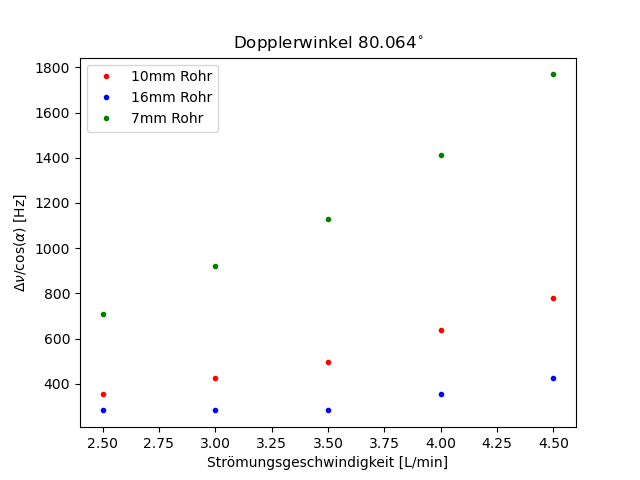
\includegraphics{1.png}
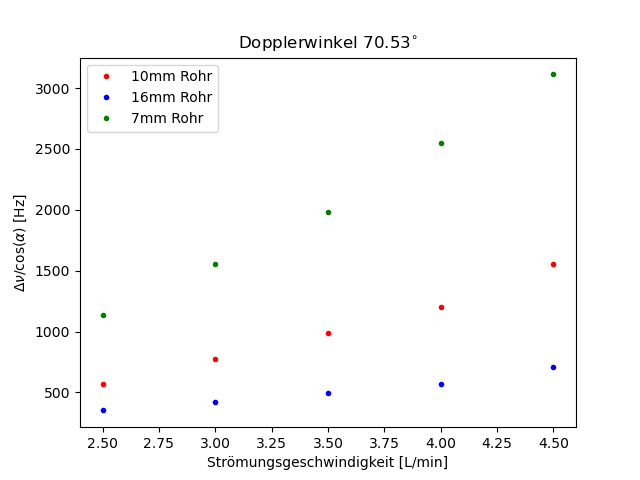
\includegraphics{2.png}
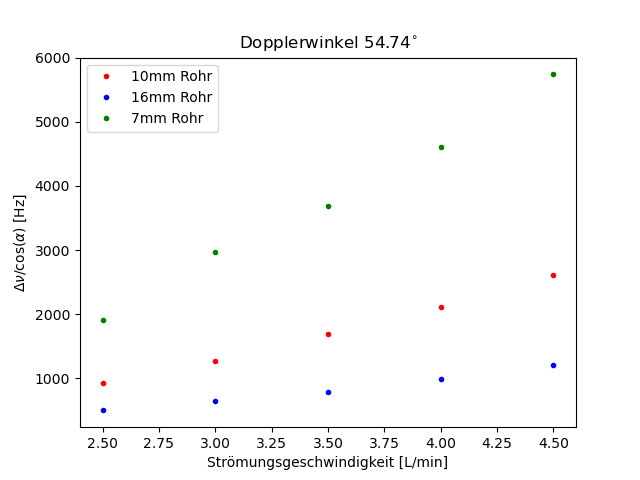
\includegraphics{3.png}

\subsection{Strömungsprofil}

Das Strömungsprofil wurde auf die bereits beschriebene Weise bestimmt.
Bei der Messung ergaben sich für verschiedene Messtiefen die Werte in \ref{tab:78}.

\noindent Diese werden werden ebenfalls graphisch dargestellt. Für jede Pumpgeschwindigkeit wird dabei eine Grafik angefertigt, in der jeweils die Strömungsgeschwindigkeit gegen die Messtiefen aufgetragen wird.

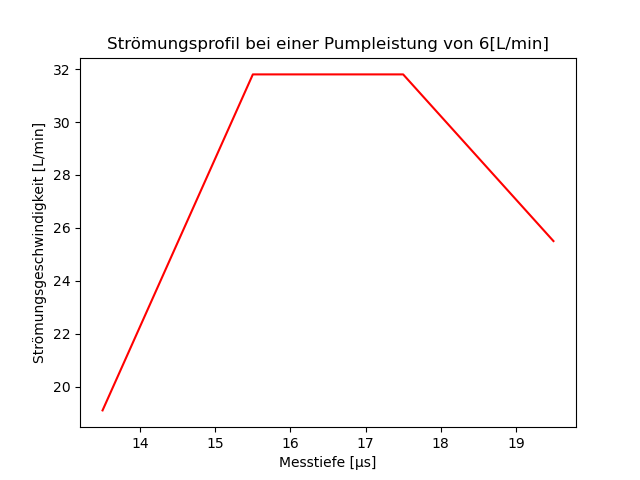
\includegraphics{4.png}
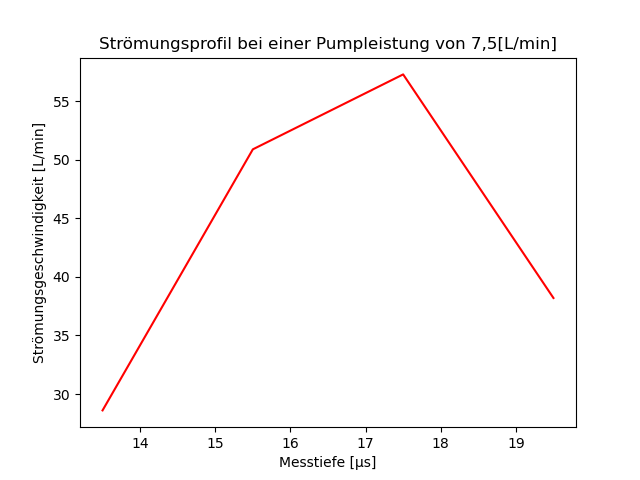
\includegraphics{5.png}

\section{Diskussion}

\subsection{Frequenzverschiebung}

\noindent Bei der Betrachtung der erhaltenen Werte für die Frequenzverschiebung fällt auf, dass sich der Betrag des Quotienten $\Delta \nu / \cos(\alpha)$ für verschiedene Dopplerwinkel $\alpha$ stark erhöt wenn der Dopplerwinkel spitzer wird. Allerdings ist auch zu beobachten, dass in allen drei Fällen der Anstieg sehr ähnlich aussieht. Außerdem wird die Steigung sehr schnell sehr groß wenn der Innendurchmesser des Rohres klein ist. Bei großen Innendurchmessern bleibt der Anstieg eher Flach in dem gewählten Messbereich. 
\noindent Bei großen Innendurchmessern war es im Experiment allerdings auch schwieriger die Strömungsgeschwindigkeiten zu messen da kleinere Veränderungen der Pumpleistung wenig bis gar keine Messbare Veränderung lieferte.
Weitere Probleme für die genaue Messbarkeit traten auch bei kleinen Innendurchmessern auf, da dort selbst die kleinsten Veränderungen der Pumpleistung große Veränderungen an den Messwerten verursachte. Diese Empfindlichkeit der Messwerte bei kleineren Innendurchmessern führte dazu, dass die Messwerte durch starke Schwankungen sehr schwierig abzulesen waren. Solche Schwankungen sind erklärbar durch die Tatsache, dass die Pumpe eventuell keine perfekt laminare Strömung erzeugt und viel mehr noch durch die Tatsache, dass es unmöglich ist die Ultraschallsonde komplett ruhig zu halten. Die Messung war wie erwähnt so empfindlich, dass kleinste Bewegungen oder Vibrationen am Tisch Schwankungen der Messwerte verursachten.

\subsection{Strömungsprofil}

Beim Vergleich der beiden Strömungsprofile fällt auf, dass der Hochpunkt der Strömungsgeschwindigkeit jeweils ungefähr in der Mitte des Rohrs, zwischen einer Messtiefe von 16 und 17 µs liegt. In beiden Fällen ist demnach am Rand eine niedrigere Strömungsgeschwindigkeit festzustellen. 
Bei dieser Messung lag eine Schwierigkeit bei der Wahl des Messbereichs. Der einstellbare Messbereich umfasste nämlich nicht den kompletten Innendurchmesser des 16mm Rohres. Deshalb wurde der Messbereich so gewählt, dass Messwerte für möglichst große Teile des Rohres genommen werden konnten.  

\section{Messwerte}

\begin{minipage}{\linewidth}
    \begin{table}[H]
        \centering
    
    \begin{tabular}{lrll}
        \toprule
        Pumpgeschwindigkeit [L/min] & Prismawinkel 15$^{\circ}$ & 30$^{\circ}$ & 60$^{\circ}$ \\
        \midrule
        2.5   &  15.9 &   13.2  &  12.4 \\ 
        3     &  19.1 &   18.1  &  17.1 \\ 
        3.5   &  22.3 &   23.1  &  22.8 \\ 
        4     &  28.7 &   28.0  &  28.5 \\ 
        4.5   &  35.0 &   36.3  &  35.2 \\    
        \bottomrule
        
    \end{tabular}
    \captionof{table}{Messwerte für Strömungsgeschwindigkeiten in [cm/s] in einem Rohr mit Innendurchmesser 10mm}
    \label{tab:1}
    \end{table}
    \end{minipage}

    \begin{minipage}{\linewidth}
        \begin{table}[H]
            \centering
        
        \begin{tabular}{lrll}
            \toprule
            Pumpgeschwindigkeit [L/min] & Prismawinkel 15$^{\circ}$ & 30$^{\circ}$ & 60$^{\circ}$ \\
            \midrule
            2.5   &  12.7  &  8.2   &  6.7   \\ 
            3     &  12.7  &  9.9   &  8.6   \\ 
            3.5   &  12.7  &  11.5  &  10.5  \\ 
            4     &  15.9  &  13.2  &  13.3  \\ 
            4.5   &  19.1  &  16.5  &  16.2  \\    
            \bottomrule
            
        \end{tabular}
        \captionof{table}{Messwerte für Strömungsgeschwindigkeiten in [cm/s] in einem Rohr mit Innendurchmesser 16mm}
        \label{tab:2}
        \end{table}
        \end{minipage}

        \begin{minipage}{\linewidth}
            \begin{table}[H]
                \centering
            
            \begin{tabular}{lrll}
                \toprule
                Pumpgeschwindigkeit [L/min] & Prismawinkel 15$^{\circ}$ & 30$^{\circ}$ & 60$^{\circ}$ \\
                \midrule
                2.5   &  31.8  &  26.4   & 25.7  \\ 
                3     &  41.4  &  36.3   & 40.0  \\ 
                3.5   &  50.9  &  46.1   & 49.5  \\ 
                4     &  63.6  &  59.3   & 61.9  \\ 
                4.5   &  79.6  &  72.5   & 77.2  \\    
                \bottomrule
                
            \end{tabular}
            \captionof{table}{Messwerte für Strömungsgeschwindigkeiten in [cm/s] in einem Rohr mit Innendurchmesser 7mm}
            \label{tab:3}
            \end{table}

            \end{minipage}
            \begin{minipage}{\linewidth}
                \begin{table}[H]
                    \centering
                
                \begin{tabular}{lrl}
                    \toprule
                    Messtiefe [µs] & Pumpgeschwindigkeit 6[L/min] & 7,5[L/min]\\
                    \midrule
                    13.5  &  19.1  &  28.6 \\
                    15.5  &  31.8  &  50.9 \\
                    17.5  &  31.8  &  57.3 \\
                    19.5  &  25.5  &  38.2 \\  
                    \bottomrule
                    
                \end{tabular}
                \captionof{table}{Messwerte für die Strömungsprofile bei verschiedenen Messtiefen in einem Rohor mit 16mm Innendurchmesser}
                \label{tab:78}
                \end{table}
                \end{minipage}

\end{document}